\documentclass[aspectratio=169]{beamer}
\usetheme{TUDelft}

% ====================================================================
% ANIMATION TOGGLE
% ====================================================================
\newif\ifanimated
\animatedtrue
\ifdefined\staticmode
  \animatedfalse
\fi
\newcommand{\cpause}{\ifanimated\pause\fi}

% Packages
\usepackage{amsmath}
\usepackage{amssymb}
\usepackage{pifont}
\usepackage{algorithm}
\usepackage{algorithmic}
\usepackage{graphicx}
\usepackage{tikz}
\usepackage{booktabs}
\usepackage{listings}
\usepackage{xcolor}
\usepackage{tcolorbox}

% Python code styling
\lstset{
    language=Python,
    basicstyle=\ttfamily\footnotesize,
    keywordstyle=\color{blue},
    commentstyle=\color{gray},
    stringstyle=\color{red},
    showstringspaces=false,
    breaklines=true,
    frame=single,
    numbers=left,
    numberstyle=\tiny\color{gray}
}

% TikZ libraries
\usetikzlibrary{shapes,arrows,positioning,calc,decorations.pathreplacing}

% Custom colors
\definecolor{sparse}{RGB}{52,152,219}    % Blue
\definecolor{dense}{RGB}{231,76,60}      % Red
\definecolor{hybrid}{RGB}{46,204,113}    % Green

\usepackage{tikz}
\usetikzlibrary{positioning, shapes, arrows, shadows, fit, calc, decorations.pathreplacing}

% Semantic Colors - One meaning per color
\definecolor{irSparse}{HTML}{3498DB}   % Sparse/BM25: Blue
\definecolor{irDense}{HTML}{E67E22}    % Dense/Embeddings: Orange
\definecolor{irRerank}{HTML}{C0392B}   % Rerank/Cross-encoder: Red
\definecolor{irHybrid}{HTML}{2ECC71}   % Hybrid/Fusion: Green
\definecolor{irANN}{HTML}{9B59B6}      % ANN/Infra: Purple
\definecolor{irInfra}{HTML}{58595B}    % General Infra: Dark Gray
\definecolor{irMuted}{HTML}{D9D9D9}    % Faint Gray

% Base Styles - Consistent Diagram Grammar
\tikzset{
    irBoxBase/.style={
        rectangle, 
        draw, 
        rounded corners=2pt, 
        minimum height=0.8cm, 
        minimum width=2cm,
        font=\small\sffamily,
        align=center,
        drop shadow={opacity=0.15},
        inner sep=5pt
    },
    irDatabase/.style={
        cylinder, 
        draw, 
        shape border rotate=90, 
        aspect=0.25, 
        minimum height=1.2cm, 
        minimum width=1cm,
        fill=irMuted!20,
        draw=irInfra,
        font=\tiny\sffamily,
        align=center
    },
    % Semantic Variants
    sparse/.style={irBoxBase, fill=irSparse!10, draw=irSparse},
    dense/.style={irBoxBase, fill=irDense!10, draw=irDense},
    rerank/.style={irBoxBase, fill=irRerank!10, draw=irRerank},
    hybrid/.style={irBoxBase, fill=irHybrid!10, draw=irHybrid},
    ann/.style={irBoxBase, fill=irANN!10, draw=irANN},
    infra/.style={irBoxBase, fill=irInfra!10, draw=irInfra},
    % Legacy support / Utility
    muted/.style={irBoxBase, fill=irMuted!20, draw=irMuted!80!black, text=irMuted!50!black},
    ghost/.style={irBoxBase, fill=white, draw=irMuted!50, text=irMuted, dashed, drop shadow={opacity=0}},
    emph/.style={draw=irRerank, thick, drop shadow={shadow xshift=0mm, shadow yshift=0mm, fill=irRerank, opacity=0.3}},
    % Arrows
    irArrowBase/.style={->, thick, >=latex, draw=irInfra},
    irLabel/.style={
        font=\tiny\itshape, 
        text=irInfra, 
        align=center, 
        text width=2.5cm, 
        inner sep=3pt
    }
}


% =========================================================
% Stage Badge System
% =========================================================
% \irStage{StageName}
\newcommand{\irStage}[1]{%
    \begin{tikzpicture}[remember picture, overlay]
        \node[
            anchor=north east,
            fill=irInfra!10,
            text=irInfra,
            font=\tiny\bfseries,
            inner sep=3pt,
            rounded corners=1pt,
            yshift=-0.5cm,
            xshift=-0.5cm
        ] at (current page.north east) {#1};
    \end{tikzpicture}%
}

% =========================================================
% Math Highlighting
% =========================================================
% \mathhl[color]{content}
\newcommand{\mathhl}[2][irDense!30]{%
    \colorbox{#1}{$\displaystyle #2$}%
}

% =========================================================
% Math Vectors
% =========================================================
\newcommand{\vs}{\mathbf{s}}

% =========================================================
% Core Box Primitives
% =========================================================
% \IRBox[width]{id}{at}{title}{subtitle}{variant}
% Default width chosen for lecture slides; override when needed.
% \IRBox[width]{id}{at}{title}{subtitle}{variant}[extra options]
\DeclareDocumentCommand{\IRBox}{O{3.5cm} m m m m m O{}}{%
    \node[#6, text width=#1, #7] (#2) at #3 {%
        \textbf{#4}%
        \if\relax\detokenize{#5}\relax
        \else\\[-1mm]\scriptsize #5%
        \fi
    };%
}

% \IRWideBox{id}{at}{width}{title}{subtitle}{variant}
\newcommand{\IRWideBox}[6]{%
    \node[#6, text width=#3] (#1) at #2 {%
        \textbf{#4}%
        \if\relax\detokenize{#5}\relax
        \else\\[-1mm]\scriptsize #5%
        \fi
    };%
}

% =========================================================
% Arrow Primitives
% =========================================================
% Safe default: left-to-right flow
% \IRArrow{from}{to}{label}
\newcommand{\IRArrow}[3]{%
    \draw[irArrowBase] (#1.east) -- node[irArrowLabelAbove] {#3} (#2.west);%
}

% Explicit left-to-right
% \IRArrowLR{from}{to}{label}
\newcommand{\IRArrowLR}[3]{%
    \draw[irArrowBase] (#1.east) -- node[irArrowLabelAbove] {#3} (#2.west);%
}

% Explicit top-to-bottom
% \IRArrowTB{from}{to}{label}
\newcommand{\IRArrowTB}[3]{%
    \draw[irArrowBase] (#1.south) -- node[irArrowLabelRight] {#3} (#2.north);%
}

% Fully explicit anchor-to-anchor path
% \IRArrowPath{from anchor}{to anchor}{label}
% Example: \IRArrowPath{a.east}{b.north}{score}
\newcommand{\IRArrowPath}[3]{%
    \draw[irArrowBase] (#1) -- node[irArrowLabelAbove] {#3} (#2);%
}

% Orthogonal elbow path
% \IRArrowElbow{from anchor}{to anchor}{label}
% Example: \IRArrowElbow{a.east}{b.north}{feedback}
\newcommand{\IRArrowElbow}[3]{%
    \draw[irArrowBase] (#1) -| node[irArrowLabelBox] {#3} (#2);%
}

% Slanted arrow for special cases only
% \IRArrowSlanted{from anchor}{to anchor}{label}{pos}{width}
\newcommand{\IRArrowSlanted}[5]{%
    \draw[irArrowBase] (#1) -- node[above, sloped, irLabel, pos=#4, text width=#5, fill=white, inner sep=1pt] {#3} (#2);%
}

% =========================================================
% Accent Elements
% =========================================================
% \IRBadge{at}{text}
\newcommand{\IRBadge}[2]{%
    \node[
        draw=irAccent,
        fill=irAccent!20,
        rounded corners=1pt,
        font=\tiny\bfseries,
        inner sep=2pt
    ] at #1 {#2};%
}

% =========================================================
% Grouping
% =========================================================
% \IRGroup{fit nodes}{label}{variant}
% Example: \IRGroup{(a)(b)(c)}{First-stage retrieval}{muted}
\newcommand{\IRGroup}[3]{%
    \node[
        irGroupBase,
        #3,
        fit=#1
    ] (group) {};
    \node[
        anchor=north west,
        font=\tiny\bfseries,
        #3
    ] at ([xshift=2pt,yshift=-2pt] group.north west) {#2};%
}

% =========================================================
% Domain-Specific Shapes
% =========================================================
% \IRDocStack{id}{at}{label}
\newcommand{\IRDocStack}[3]{%
    \node[irDocStack] (#1) at #2 {#3};%
}

% \IRDatabase{id}{at}{label}
\newcommand{\IRDatabase}[3]{%
    \node[irDatabase] (#1) at #2 {#3};%
}

% =========================================================
% Layout Helpers
% =========================================================
% \IRPipelineTier{id}{at}{text}{label}{variant}
\newcommand{\IRPipelineTier}[5]{%
    \IRBox{#1}{#2}{#3}{}{#5}[]
    \node[anchor=west, irLabel, xshift=0.5cm] at (#1.east) {#4};%
}

% \IRTelescopeTier{id}{at}{width}{text}{variant}
\newcommand{\IRTelescopeTier}[5]{%
    \node[
        irTelescopeBase,
        #5,
        minimum width=#3
    ] (#1) at #2 {#4};%
}

% \IRStep{id}{at}{title}{subtitle}{variant}
% Creates a numbered step badge left of a box.
\newcommand{\IRStep}[5]{%
    \node[
        circle,
        draw=irAccent,
        fill=irAccent!20,
        font=\tiny\bfseries,
        inner sep=2pt
    ] (#1_num) at #2 {#1};
    \node[
        #5,
        text width=3.5cm,
        right=1.5cm of #1_num
    ] (#1) {%
        \textbf{#3}%
        \if\relax\detokenize{#4}\relax
        \else\\[-1mm]\scriptsize #4%
        \fi
    };
    \draw[irArrowBase, thin] (#1_num.east) -- (#1.west);%
}


% Title information
\title[Ranking Models]{Information Retrieval Ranking Models}
\subtitle{Lecture 3: Sparse Ranking Methods (BM25, Language Models, Query Expansion)}
\author{Avishek Anand}
\institute{Information Retrieval}
\date{\today}

\begin{document}

% Title slide
\begin{frame}
\titlepage
\end{frame}

\begin{frame}{Outline}
\tableofcontents
\end{frame}

% ====================================================================
% SECTION 1: FROM VECTOR SPACE TO PROBABILISTIC RANKING
% ====================================================================
\section{From Vector Space to Probabilistic Ranking}

\begin{frame}[plain]
\sectionpage
\end{frame}

\begin{frame}{Recap: What We Know}
\begin{block}{Vector Space Model (Lecture 1)}
\begin{itemize}
    \item Documents and queries as vectors in term space
    \item Similarity measured by cosine distance
    \item Foundation for understanding term-based retrieval
\end{itemize}
\end{block}

\begin{block}{Indexing (Lecture 2)}
\begin{itemize}
    \item Inverted index: term $\to$ posting list (docID, tf, positions)
    \item Accumulator-based scoring: only touch documents with term overlap
    \item Dense indexing: IVF+PQ for semantic vectors
\end{itemize}
\end{block}

\begin{alertblock}{Today's Question}
We can store and retrieve efficiently. But \textbf{how do we score?}
\end{alertblock}
\end{frame}

\begin{frame}[shrink=5]{The Probability Ranking Principle (PRP)}
\begin{block}{Theorem (Robertson, 1977)}
If documents are ranked by decreasing probability of relevance given the query, then the expected effectiveness of the system is maximized---under the assumption of independent relevance.
\end{block}

\vspace{1em}

\textbf{Formally:} Rank by $P(\text{relevant} \mid q, d)$

\vspace{1em}

\textbf{Implications:}
\begin{itemize}
    \item Gives a \textbf{theoretical justification} for probabilistic scoring
    \item All scoring functions (TF-IDF, BM25, LM) are approximations of this ideal
    \item Independence assumption is strong---violated in practice (documents are correlated)
\end{itemize}

\vspace{0.5em}

\begin{exampleblock}{Key Insight}
The PRP tells us \emph{what} to optimize. BM25 and Language Models tell us \emph{how}.
\end{exampleblock}
\end{frame}

\begin{frame}[shrink=5]{The Ranking Problem}
\begin{block}{Formal Definition}
\textbf{Given:}
\begin{itemize}
    \item Query $q$ (sequence of terms)
    \item Document collection $D$
    \item Inverted index (from Lecture 2)
\end{itemize}

\vspace{0.5em}
\textbf{Return:} Ranked list scored by relevance $P(\text{relevant}|q,d)$
\end{block}

\vspace{1em}

\begin{exampleblock}{Key Insight}
Not all term matches are equal:
\begin{itemize}
    \item Rare terms (``syzygy'') more informative than common (``the'')
    \item Term frequency matters, but with diminishing returns
    \item Document length affects scoring
\end{itemize}
\end{exampleblock}
\end{frame}

\begin{frame}{Term Weighting: TF-IDF}
\begin{columns}
\begin{column}{0.5\textwidth}
\textbf{Term Frequency (TF)}
\begin{itemize}
    \item More occurrences $\rightarrow$ more important
    \item $\text{tf}(t,d) = \text{count}(t,d)$
\end{itemize}

\vspace{1em}

\textbf{Inverse Document Frequency (IDF)}
\begin{itemize}
    \item Rare terms $\rightarrow$ more discriminative
    \item $\text{idf}(t) = \log\frac{N}{\text{df}_t}$
\end{itemize}
\end{column}

\begin{column}{0.5\textwidth}
\begin{block}{Combined Score}
$$\text{TF-IDF}(t,d) = \text{tf}(t,d) \times \text{idf}(t)$$
\end{block}

\vspace{1em}

\begin{alertblock}{Problem}
Linear TF growth unrealistic:
\begin{itemize}
    \item 100 occurrences $\neq$ 100$\times$ more relevant than 1
    \item Need saturation
\end{itemize}
\end{alertblock}
\end{column}
\end{columns}
\end{frame}

\begin{frame}{TF-IDF Example}
\textbf{Query:} ``information retrieval'' \quad ($N = 100{,}000$ documents)

\vspace{1em}

\begin{table}
\centering
\small
\begin{tabular}{lccccc}
\toprule
\textbf{Term} & \textbf{Doc 1} & \textbf{Doc 2} & \textbf{df} & \textbf{IDF} & \textbf{Weight} \\
\midrule
information & 3 & 1 & 5000 & 1.30 & High TF \\
retrieval & 2 & 0 & 500 & 2.30 & High IDF \\
the & 20 & 15 & 50000 & 0.30 & Low IDF \\
\bottomrule
\end{tabular}
\end{table}

\vspace{1em}

\begin{block}{Observation}
\begin{itemize}
    \item ``retrieval'' gets high weight (rare term)
    \item ``the'' downweighted despite frequency (common term)
    \item But TF still grows linearly $\rightarrow$ need saturation
\end{itemize}
\end{block}
\end{frame}

% ====================================================================
% SECTION 2: BM25
% ====================================================================
\section{BM25: The Probabilistic Standard}

\begin{frame}[plain]
\sectionpage
\end{frame}

\begin{frame}{Motivation: TF Saturation}
\begin{columns}
\begin{column}{0.5\textwidth}
\textbf{Observation:}
\begin{itemize}
    \item Relevance increases with TF
    \item But saturates quickly
\end{itemize}

\vspace{1em}

\textbf{Example:}
\begin{itemize}
    \item ``algorithm'' 5$\times$ vs. 50$\times$ 
    \item 5$\rightarrow$10 is meaningful
    \item 45$\rightarrow$50 barely noticeable
\end{itemize}
\end{column}

\begin{column}{0.5\textwidth}
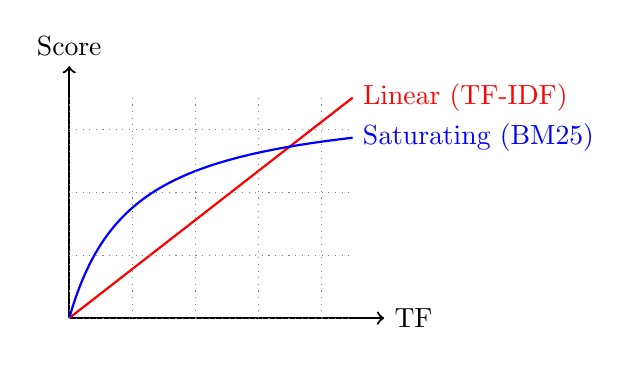
\begin{tikzpicture}[scale=0.8]
    \draw[->, thick] (0,0) -- (5,0) node[right] {TF};
    \draw[->, thick] (0,0) -- (0,4) node[above] {Score};
    \draw[red, thick] (0,0) -- (4.5,3.5) node[right] {Linear (TF-IDF)};
    \draw[blue, thick, domain=0:4.5, samples=100] 
        plot (\x, {3.5*\x/(1+\x)}) node[right] {Saturating (BM25)};
    \draw[gray, dotted] (0,0) grid (4.5,3.5);
\end{tikzpicture}

\end{column}
\end{columns}

\vspace{1em}

\begin{alertblock}{Need}
Non-linear TF component that saturates gracefully
\end{alertblock}
\end{frame}

\begin{frame}{BM25 Formula}
\begin{block}{Complete Formula}
$$\text{BM25}(q,d) = \sum_{t \in q} \text{IDF}(t) \cdot \frac{f(t,d) \cdot (k_1+1)}{f(t,d) + k_1 \cdot \left(1-b+b \cdot \frac{|d|}{\text{avgdl}}\right)}$$
\end{block}

\vspace{1em}

\textbf{Three components:}
\begin{enumerate}
    \item \textbf{IDF:} Term importance (like TF-IDF)
    \item \textbf{Saturating TF:} Non-linear term frequency
    \item \textbf{Length normalization:} Penalize long documents
\end{enumerate}

\vspace{1em}

\begin{center}
\textbf{Standard parameters: $k_1 = 1.2$, $b = 0.75$}
\end{center}
\end{frame}

\begin{frame}{BM25 Component 1: IDF}
\begin{block}{IDF Formula}
$$\text{IDF}(t) = \log\frac{N - \text{df}_t + 0.5}{\text{df}_t + 0.5}$$
\end{block}

where:
\begin{itemize}
    \item $N$ = total number of documents
    \item $\text{df}_t$ = document frequency of term $t$
\end{itemize}

\vspace{1em}

\textbf{Properties:}
\begin{itemize}
    \item Similar to TF-IDF but probabilistically motivated
    \item Can be negative for very common terms ($\text{df} > N/2$)
    \item Rare terms get high positive IDF
    \item Common terms get low or negative IDF
\end{itemize}
\end{frame}

\begin{frame}{BM25 Component 2: Saturating TF}
\begin{block}{Saturating TF Formula}
$$\frac{f(t,d) \cdot (k_1+1)}{f(t,d) + k_1}$$
\end{block}

\textbf{Parameter $k_1$ (typically 1.2--2.0):}
\begin{itemize}
    \item $k_1 \to 0$: Boolean matching (TF doesn't matter)
    \item $k_1 \to \infty$: Linear TF (like TF-IDF)
    \item $k_1 = 1.2$: Moderate saturation (standard)
\end{itemize}

\vspace{1em}

\begin{columns}
\begin{column}{0.5\textwidth}
\small
\begin{tabular}{ccc}
\toprule
\textbf{TF} & \textbf{$k_1=1.2$} & \textbf{$k_1=2.0$} \\
\midrule
1 & 0.55 & 0.67 \\
5 & 1.53 & 1.67 \\
10 & 1.79 & 1.83 \\
50 & 1.98 & 1.96 \\
\bottomrule
\end{tabular}
\end{column}

\begin{column}{0.5\textwidth}
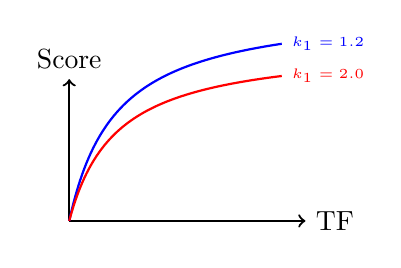
\begin{tikzpicture}[scale=0.6]
    \draw[->, thick] (0,0) -- (5,0) node[right] {TF};
    \draw[->, thick] (0,0) -- (0,3) node[above] {Score};
    \draw[blue, thick, domain=0:4.5, samples=100] 
        plot (\x, {2.5*\x*2.2/(1.2*\x+1.2)}) node[right] {\tiny $k_1=1.2$};
    \draw[red, thick, domain=0:4.5, samples=100] 
        plot (\x, {2.5*\x*3/(2*\x+2)}) node[right] {\tiny $k_1=2.0$};
\end{tikzpicture}

\end{column}
\end{columns}
\end{frame}

\begin{frame}[shrink=5]{BM25 Component 3: Length Normalization}
\begin{block}{Length Normalization Term}
$$1 - b + b \cdot \frac{|d|}{\text{avgdl}}$$
\end{block}

\textbf{Parameter $b$ (typically 0.75):}
\begin{itemize}
    \item $b = 0$: No length normalization
    \item $b = 1$: Full normalization (penalize long docs heavily)
    \item $b = 0.75$: Partial normalization (standard)
\end{itemize}

\vspace{1em}

\textbf{Why needed:}
\begin{itemize}
    \item Long documents have more terms just by chance
    \item Should we penalize or not? Depends on collection
    \item $b$ controls the trade-off
\end{itemize}
\end{frame}


% ====================================================================
% NEW: WORKED BM25 EXAMPLE (END-TO-END)
% ====================================================================

\begin{frame}[shrink=10]{Worked Example: Full BM25 Scoring}
\textbf{Query:} ``quantum algorithm'' \quad $N = 100{,}000$, avgdl $= 500$

\vspace{0.5em}

\textbf{Two candidate documents:}
\begin{itemize}
    \item Doc A: 300 words. ``quantum'' appears 5$\times$, ``algorithm'' appears 3$\times$.
    \item Doc B: 800 words. ``quantum'' appears 8$\times$, ``algorithm'' appears 1$\times$.
\end{itemize}

\textbf{Collection stats:} df(quantum) $= 200$, df(algorithm) $= 5{,}000$

\vspace{0.5em}

\textbf{Step 1: Compute IDF.}
\begin{align*}
\text{IDF}(\text{quantum}) &= \log\frac{100000 - 200 + 0.5}{200 + 0.5} = \log\frac{99800.5}{200.5} = \log(497.8) = \mathbf{6.21} \\
\text{IDF}(\text{algorithm}) &= \log\frac{100000 - 5000 + 0.5}{5000 + 0.5} = \log\frac{95000.5}{5000.5} = \log(19.0) = \mathbf{2.94}
\end{align*}
\end{frame}

\begin{frame}[shrink=10]{Worked Example: Full BM25 Scoring (cont.)}
\textbf{Step 2: Compute scores.} ($k_1 = 1.2$, $b = 0.75$, avgdl $= 500$)

\vspace{0.5em}

\textbf{Doc A} ($|d| = 300$): \quad norm $= 1 - 0.75 + 0.75 \cdot \frac{300}{500} = 0.70$

\vspace{-0.3em}
{\small
\begin{align*}
\text{quantum:} &\quad \frac{5 \times 2.2}{5 + 1.2 \times 0.70} = \frac{11.0}{5.84} = 1.88 \\
\text{algorithm:} &\quad \frac{3 \times 2.2}{3 + 1.2 \times 0.70} = \frac{6.6}{3.84} = 1.72 \\
\text{BM25}(q, A) &= 6.21 \times 1.88 + 2.94 \times 1.72 = 11.67 + 5.06 = \mathbf{16.73}
\end{align*}
}

\textbf{Doc B} ($|d| = 800$): \quad norm $= 1 - 0.75 + 0.75 \cdot \frac{800}{500} = 1.45$

\vspace{-0.3em}
{\small
\begin{align*}
\text{quantum:} &\quad \frac{8 \times 2.2}{8 + 1.2 \times 1.45} = \frac{17.6}{9.74} = 1.81 \\
\text{algorithm:} &\quad \frac{1 \times 2.2}{1 + 1.2 \times 1.45} = \frac{2.2}{2.74} = 0.80 \\
\text{BM25}(q, B) &= 6.21 \times 1.81 + 2.94 \times 0.80 = 11.24 + 2.35 = \mathbf{13.59}
\end{align*}
}

\begin{exampleblock}{Result: Doc A (16.73) $>$ Doc B (13.59)}
Doc A wins despite fewer ``quantum'' hits. Why? (1) Shorter doc $\to$ less length penalty. (2) More ``algorithm'' hits $\to$ both query terms well-covered.
\end{exampleblock}
\end{frame}

\begin{frame}{BM25 Example: Effect of Document Length}
\textbf{Scenario:} Term appears 20 times, $k_1=1.2$, $b=0.75$, avgdl=1000

\vspace{1em}

\begin{columns}
\begin{column}{0.5\textwidth}
\textbf{Short Document (500 words)}
\begin{align*}
\text{norm} &= 1 - 0.75 + 0.75 \cdot \frac{500}{1000} \\
&= 0.625 \\
\text{TF component} &= \frac{20 \cdot 2.2}{20 + 1.2 \cdot 0.625} \\
&= \frac{44}{20.75} = 2.12
\end{align*}
\end{column}

\begin{column}{0.5\textwidth}
\textbf{Long Document (2000 words)}
\begin{align*}
\text{norm} &= 1 - 0.75 + 0.75 \cdot \frac{2000}{1000} \\
&= 1.75 \\
\text{TF component} &= \frac{20 \cdot 2.2}{20 + 1.2 \cdot 1.75} \\
&= \frac{44}{22.1} = 1.99
\end{align*}
\end{column}
\end{columns}

\vspace{1em}

\begin{alertblock}{Observation}
Same TF, but short document scores higher due to length penalty
\end{alertblock}
\end{frame}

\begin{frame}{BM25 Example: Rare vs. Common Terms}
\textbf{Collection:} $N = 100{,}000$ documents

\vspace{1em}

\begin{table}
\centering
\begin{tabular}{lccc}
\toprule
\textbf{Term} & \textbf{df} & \textbf{IDF} & \textbf{Interpretation} \\
\midrule
quantum & 100 & 6.21 & Very discriminative \\
algorithm & 5{,}000 & 2.99 & Moderately discriminative \\
system & 50{,}000 & $-0.41$ & Not discriminative \\
the & 99{,}000 & $-6.21$ & Actively harmful \\
\bottomrule
\end{tabular}
\end{table}

\vspace{1em}

\begin{block}{Key Insight}
IDF difference drives discrimination:
\begin{itemize}
    \item Rare terms dominate scoring
    \item Common terms contribute little or negatively
    \item Matches on ``quantum'' worth $\sim$15$\times$ matches on ``system''
\end{itemize}
\end{block}
\end{frame}

\begin{frame}[shrink=5]{BM25F: Fielded Documents}
\begin{block}{Motivation}
Real documents have \textbf{fields}: title, abstract, body, URL, anchor text. \\
A match in the title is worth more than a match in the body.
\end{block}

\vspace{0.5em}

\begin{block}{BM25F Formula (Simplified)}
Replace raw TF with a \textbf{weighted sum across fields}:
$$\tilde{f}(t, d) = \sum_{z \in \text{fields}} w_z \cdot \frac{f(t, d_z)}{1 - b_z + b_z \cdot \frac{|d_z|}{\text{avgdl}_z}}$$
Then plug $\tilde{f}$ into standard BM25 in place of $f(t,d)$.
\end{block}

\vspace{0.5em}

\textbf{Parameters per field:}
\begin{itemize}
    \item $w_z$: field weight (title $w = 5$, body $w = 1$, URL $w = 2$)
    \item $b_z$: per-field length normalization
\end{itemize}

\vspace{0.5em}

\begin{exampleblock}{Used In}
Elasticsearch, Solr, Bing, and most production web search engines
\end{exampleblock}
\end{frame}

\begin{frame}{BM25 Parameter Tuning Guidelines}
\begin{block}{Standard Defaults}
$k_1 = 1.2$, $b = 0.75$ (works well for many collections)
\end{block}

\vspace{1em}

\begin{columns}
\begin{column}{0.5\textwidth}
\textbf{When to adjust $k_1$:}
\begin{itemize}
    \item \textbf{Verbose collections} (news, articles) \\
    $\rightarrow$ Higher $k_1$ (1.5--2.0)
    \item \textbf{Keyword collections} (tweets, queries) \\
    $\rightarrow$ Lower $k_1$ (0.8--1.2)
\end{itemize}
\end{column}

\begin{column}{0.5\textwidth}
\textbf{When to adjust $b$:}
\begin{itemize}
    \item \textbf{Variable-length docs} (web pages) \\
    $\rightarrow$ Higher $b$ (0.8--0.9)
    \item \textbf{Uniform-length docs} (abstracts) \\
    $\rightarrow$ Lower $b$ (0.5--0.7)
\end{itemize}
\end{column}
\end{columns}

\vspace{1em}

\begin{alertblock}{In Lecture 6 (Learning to Rank)}
You'll learn to tune these parameters systematically using labeled data
\end{alertblock}
\end{frame}

% ====================================================================
% SECTION 3: QUERY EXPANSION
% ====================================================================
\section{Query Expansion and Pseudo Relevance Feedback}

\begin{frame}[plain]
\sectionpage
\end{frame}

\begin{frame}{The Vocabulary Mismatch Problem}
\begin{exampleblock}{Core Issue}
Queries and relevant documents use different vocabulary:
\end{exampleblock}

\vspace{1em}

\begin{columns}
\begin{column}{0.48\textwidth}
\textbf{Medical Domain}
\begin{itemize}
    \item Query: ``heart attack''
    \item Document: ``myocardial infarction''
\end{itemize}

\vspace{0.5em}

\textbf{Technical Domain}
\begin{itemize}
    \item Query: ``ML''
    \item Document: ``machine learning''
\end{itemize}
\end{column}

\begin{column}{0.48\textwidth}
\textbf{General Domain}
\begin{itemize}
    \item Query: ``elderly care''
    \item Document: ``geriatric nursing''
\end{itemize}

\vspace{0.5em}

\textbf{Result}
\begin{itemize}
    \item BM25 score = 0
    \item Relevant doc not retrieved
\end{itemize}
\end{column}
\end{columns}

\vspace{1em}

\begin{alertblock}{Sparse Retrieval Limitation}
Exact term matching only --- no semantic understanding
\end{alertblock}

\vspace{0.5em}

\textit{(Fully addressed by Dense Retrieval in Lecture 5)}
\end{frame}

\begin{frame}[shrink=5]{Relevance Feedback Overview}
\begin{block}{Explicit Relevance Feedback}
User marks documents as relevant/non-relevant
\begin{itemize}
    \item \textcolor{red}{\ding{55}} Impractical: users won't give feedback
    \item \textcolor{red}{\ding{55}} Chicken-and-egg: need good initial results
\end{itemize}
\end{block}

\vspace{1em}

\begin{block}{Pseudo Relevance Feedback (PRF)}
\textbf{Assumption:} Top-$k$ retrieved documents are relevant
\begin{itemize}
    \item \textcolor{green}{\checkmark} No user interaction needed
    \item \textcolor{green}{\checkmark} Automatic query expansion
    \item \textcolor{red}{\ding{55}} Risk: If assumption fails $\rightarrow$ query drift
\end{itemize}
\end{block}

\vspace{1em}

\textbf{Process:}
\begin{enumerate}
    \item Retrieve initial results with original query
    \item Extract terms from top-$k$ documents
    \item Expand query with these terms
    \item Re-retrieve with expanded query
\end{enumerate}
\end{frame}

\begin{frame}[shrink=10]{Rocchio Algorithm}
\begin{block}{Historical Context}
Classic PRF method from 1971, vector space approach
\end{block}

\begin{block}{Formula}
$$\vec{q}_{\text{new}} = \alpha \vec{q}_{\text{original}} + \beta \frac{1}{|R|}\sum_{d \in R} \vec{d} - \gamma \frac{1}{|NR|}\sum_{d \in NR} \vec{d}$$
\end{block}

\textbf{Parameters:}
\begin{itemize}
    \item $\alpha = 1$: Keep original query (always)
    \item $\beta = 0.75$: Weight toward positive examples
    \item $\gamma = 0.15$: Weight away from negative examples
    \item In PRF: $\gamma = 0$ (no negative feedback available)
\end{itemize}

\vspace{0.5em}

\textbf{Geometric Intuition:} Move query vector toward centroid of relevant documents, away from non-relevant.
\end{frame}

\begin{frame}{Rocchio: Geometric Intuition}
\begin{center}
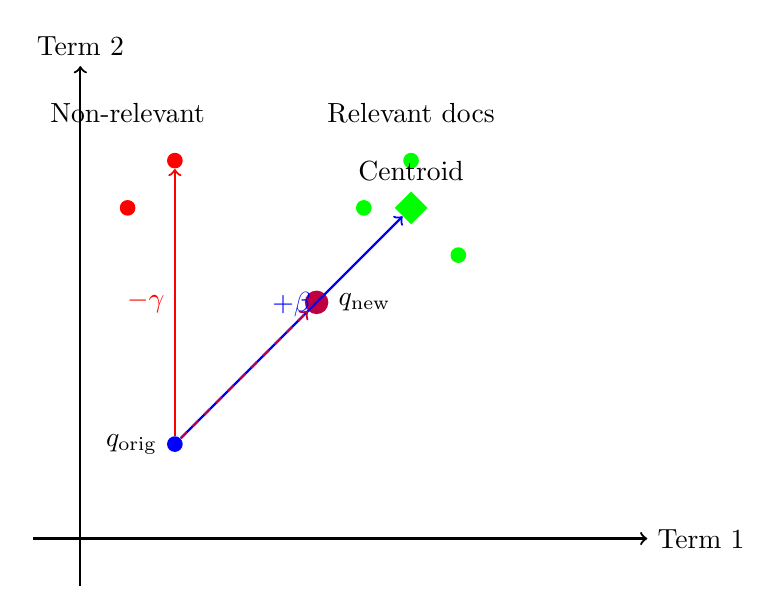
\begin{tikzpicture}[scale=1.2]
    \draw[->, thick] (-0.5,0) -- (6,0) node[right] {Term 1};
    \draw[->, thick] (0,-0.5) -- (0,5) node[above] {Term 2};
    \node[circle, fill=blue, inner sep=2pt, label=left:$q_{\text{orig}}$] (q) at (1,1) {};
    \node[circle, fill=green, inner sep=2pt] (d1) at (3,3.5) {};
    \node[circle, fill=green, inner sep=2pt] (d2) at (4,3) {};
    \node[circle, fill=green, inner sep=2pt] (d3) at (3.5,4) {};
    \node at (3.5,4.5) {Relevant docs};
    \node[diamond, fill=green, inner sep=3pt, label=above:Centroid] (c) at (3.5,3.5) {};
    \node[circle, fill=red, inner sep=2pt] (n1) at (1,4) {};
    \node[circle, fill=red, inner sep=2pt] (n2) at (0.5,3.5) {};
    \node at (0.5,4.5) {Non-relevant};
    \node[circle, fill=purple, inner sep=3pt, label=right:$q_{\text{new}}$] (qn) at (2.5,2.5) {};
    \draw[->, thick, blue] (q) -- (c) node[midway, above] {$+\beta$};
    \draw[->, thick, red] (q) -- (n1) node[midway, left] {$-\gamma$};
    \draw[->, thick, purple, dashed] (q) -- (qn);
\end{tikzpicture}

\end{center}

\textbf{Movement:} Original query shifts toward relevant docs, away from non-relevant
\end{frame}

\begin{frame}[shrink=5]{Rocchio Limitations}
\begin{alertblock}{\ding{55} Why Not Standard Anymore?}
\begin{enumerate}
    \item \textbf{Requires vector space representation}
    \begin{itemize}
        \item All terms contribute (even noisy ones)
        \item No principled term selection
    \end{itemize}
    \item \textbf{No probabilistic foundation}
    \begin{itemize}
        \item Weights based on geometry, not probability
    \end{itemize}
    \item \textbf{Empirically outperformed} by RM3
\end{enumerate}
\end{alertblock}

\vspace{1em}

\begin{block}{Modern Usage}
Mainly historical importance --- RM3 is the standard for classical PRF
\end{block}
\end{frame}

\begin{frame}{RM3: Relevance Model 3}
\begin{block}{Foundation}
Probabilistic query expansion using language modeling framework
\end{block}

\vspace{1em}

\textbf{Two-stage process:}

\begin{enumerate}
    \item \textbf{Estimate Relevance Model}
    $$P(w|R) \propto \sum_{d \in R} P(w|d) \cdot P(d|q)$$
    \begin{itemize}
        \item For each word $w$, estimate probability from ``relevance''
        \item Weight by how relevant each doc appears: $P(d|q)$ from initial retrieval
        \item Select top \texttt{fb\_terms} words by $P(w|R)$
    \end{itemize}
    
    \item \textbf{Interpolate with Original Query}
    $$P(w|Q_{\text{new}}) = (1-\lambda) \cdot P(w|Q_{\text{original}}) + \lambda \cdot P(w|R)$$
    \begin{itemize}
        \item $\lambda$ typically 0.5--0.8: balance original vs. expansion
    \end{itemize}
\end{enumerate}
\end{frame}

\begin{frame}[shrink=5]{RM3: Key Parameters}
\begin{block}{fb\_docs (Feedback Documents): 3--10}
How many top documents to use for expansion
\begin{itemize}
    \item Too few: May miss relevant terms. Too many: Risk non-relevant docs.
    \item \textbf{Standard:} 10
\end{itemize}
\end{block}

\begin{block}{fb\_terms (Feedback Terms): 10--20}
How many expansion terms to add
\begin{itemize}
    \item Too few: Limited benefit. Too many: Noise.
    \item \textbf{Standard:} 10
\end{itemize}
\end{block}

\begin{block}{$\lambda$ (Interpolation Weight): 0.5--0.8}
Original vs. expansion weight
\begin{itemize}
    \item Lower (0.5): Trust original query more
    \item Higher (0.8): Trust expansion more
\end{itemize}
\end{block}
\end{frame}

\begin{frame}[shrink=5]{RM3 Example}
\textbf{Original Query:} ``machine learning''

\vspace{0.5em}

\textbf{Top-3 Retrieved Documents (fb\_docs=3):}
\begin{enumerate}
    \item ``Neural networks and deep learning algorithms...''
    \item ``Supervised machine learning techniques...''
    \item ``Machine learning applications in AI...''
\end{enumerate}

\vspace{0.5em}

\textbf{Extracted Terms (fb\_terms=5):}
\begin{itemize}
    \item neural (P=0.15), deep (P=0.12), supervised (P=0.10), algorithms (P=0.09), AI (P=0.08)
\end{itemize}

\vspace{0.5em}

\textbf{Expanded Query ($\lambda=0.6$):}
\\
``machine learning neural deep supervised algorithms AI''
\end{frame}


% ====================================================================
% NEW SECTION: LLM-BASED QUERY EXPANSION
% ====================================================================

\begin{frame}{Beyond PRF: Modern Query Expansion Strategies}
\begin{center}
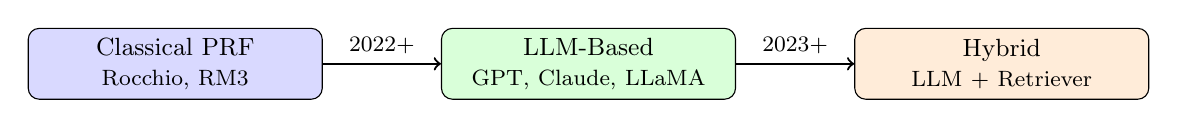
\begin{tikzpicture}[
    node distance=1.2cm,
    box/.style={rectangle, draw, rounded corners, text width=3.5cm, align=center, minimum height=0.9cm, font=\small},
    arrow/.style={->, thick}
]
    \node[box, fill=blue!15] (classical) {Classical PRF\\{\footnotesize Rocchio, RM3}};
    \node[box, fill=green!15, right=1.5cm of classical] (llm) {LLM-Based\\{\footnotesize GPT, Claude, LLaMA}};
    \node[box, fill=orange!15, right=1.5cm of llm] (hybrid) {Hybrid\\{\footnotesize LLM + Retriever}};
    
    \draw[arrow] (classical) -- (llm) node[midway, above, font=\footnotesize] {2022+};
    \draw[arrow] (llm) -- (hybrid) node[midway, above, font=\footnotesize] {2023+};
\end{tikzpicture}

\end{center}

\vspace{1em}

\begin{block}{Key Insight}
LLMs have \textbf{parametric knowledge} --- they can generate expansion terms without retrieving any documents first. No risk of PRF's ``bad top-$k$'' problem!
\end{block}
\end{frame}

\begin{frame}[shrink=5]{Strategy 1: LLM Synonym \& Paraphrase Generation}
\begin{block}{Idea}
Ask an LLM to generate synonyms, related terms, or paraphrases of the query.
\end{block}

\vspace{0.5em}

\textbf{Prompt:}
\begin{tcolorbox}[colback=gray!10, colframe=gray!50, fontupper=\small\ttfamily]
Given the search query: "heart attack symptoms"\\
Generate 5 alternative phrasings and medical synonyms that a relevant document might use.\\
Return only the terms, one per line.
\end{tcolorbox}

\vspace{0.5em}

\textbf{LLM Output:}
\begin{itemize}
    \item myocardial infarction signs
    \item cardiac arrest warning indicators
    \item chest pain emergency symptoms
    \item coronary event presentation
    \item acute heart failure signs
\end{itemize}

\vspace{0.5em}

\textbf{Expanded BM25 query:} ``heart attack symptoms myocardial infarction cardiac coronary chest pain''

\begin{exampleblock}{Advantage}
Bridges the exact vocabulary gap that BM25 cannot handle on its own
\end{exampleblock}
\end{frame}

\begin{frame}[shrink=5]{Strategy 2: Hypothetical Document Generation (HyDE)}
\begin{block}{Core Idea (Gao et al., 2023)}
Ask the LLM to \textbf{generate a hypothetical relevant document}, then use its embedding for dense retrieval or extract its terms for sparse expansion.
\end{block}

\vspace{0.5em}

\textbf{Prompt:}
\begin{tcolorbox}[colback=gray!10, colframe=gray!50, fontupper=\small\ttfamily]
Write a short paragraph that would be a perfect answer to the question: "What causes ocean acidification?"
\end{tcolorbox}

\vspace{0.5em}

\textbf{LLM Output:}
\begin{quote}
\small\itshape
``Ocean acidification is primarily caused by the absorption of atmospheric carbon dioxide (CO$_2$) by seawater. When CO$_2$ dissolves, it forms carbonic acid, which lowers the pH of the ocean. This process threatens marine organisms with calcium carbonate shells, such as corals and mollusks...''
\end{quote}

\vspace{0.5em}

\textbf{For Sparse:} Extract key terms $\to$ ``carbonic acid'', ``calcium carbonate'', ``pH'', ``seawater'', ``corals''

\textbf{For Dense:} Embed the hypothetical doc $\to$ use as query vector (Lecture 5)
\end{frame}

\begin{frame}[shrink=5]{Strategy 3: Chain-of-Thought Query Decomposition}
\begin{block}{Idea}
Complex queries benefit from being broken into sub-queries that each retrieve different evidence.
\end{block}

\vspace{0.5em}

\textbf{Prompt:}
\begin{tcolorbox}[colback=gray!10, colframe=gray!50, fontupper=\small\ttfamily]
I need to answer: "How did the 2008 financial crisis affect European housing markets?"\\
Break this into 3-4 simpler search queries that together would cover the full answer.
\end{tcolorbox}

\vspace{0.5em}

\textbf{LLM Output:}
\begin{enumerate}
    \item ``2008 financial crisis causes subprime mortgage''
    \item ``European housing prices 2008 2009 decline''
    \item ``EU bank bailouts housing market impact''
    \item ``European mortgage lending regulations post-crisis''
\end{enumerate}

\vspace{0.5em}

\begin{block}{Pipeline}
Run BM25 on each sub-query $\to$ merge results $\to$ better recall than single complex query
\end{block}
\end{frame}

\begin{frame}[shrink=10]{Strategy 4: Query2Doc (Wang et al., 2023)}
\begin{block}{Idea}
Generate a pseudo-document with an LLM, \textbf{prepend it to the original query}, and run BM25 on the concatenation.
\end{block}

\vspace{0.5em}

\textbf{Original query:} ``dark matter detection methods''

\textbf{LLM-generated pseudo-doc:}
\begin{quote}
\small\itshape
``Dark matter detection experiments include direct detection using cryogenic detectors, indirect detection through gamma-ray observations, and collider searches at the Large Hadron Collider...''
\end{quote}

\textbf{Expanded query to BM25:} original query + pseudo-doc text

\vspace{0.5em}

\begin{columns}
\begin{column}{0.48\textwidth}
\textbf{\textcolor{green}{\checkmark} Advantages:}
\begin{itemize}
    \item Drops into any BM25 system
    \item No retrieval needed first
    \item LLM runs once per query
\end{itemize}
\end{column}
\begin{column}{0.48\textwidth}
\textbf{\textcolor{red}{\ding{55}} Risks:}
\begin{itemize}
    \item LLM hallucinations add noise
    \item Longer ``query'' = slower
    \item Need to weight original vs.\ generated text
\end{itemize}
\end{column}
\end{columns}
\end{frame}

\begin{frame}{Comparison: Classical vs. LLM Query Expansion}
\begin{table}
\centering
\small
\begin{tabular}{lll}
\toprule
\textbf{Aspect} & \textbf{Classical (RM3)} & \textbf{LLM-Based} \\
\midrule
Knowledge source & Top-$k$ retrieved docs & Parametric (training data) \\
Failure mode & Query drift (bad top-$k$) & Hallucination \\
Latency & Fast (stats only) & Slower (LLM inference) \\
Cost & Free & API cost / GPU \\
Domain knowledge & Needs in-domain corpus & Pre-trained, zero-shot \\
Cold-start & Fails (empty index) & Works (no index needed) \\
Interpretability & Terms from real docs & Generated terms \\
\bottomrule
\end{tabular}
\end{table}

\vspace{1em}

\begin{exampleblock}{Best Practice (2024+)}
\textbf{Combine both:} Use LLM expansion to improve the initial retrieval, then apply RM3 on the (now better) top-$k$ results. The two methods are complementary.
\end{exampleblock}
\end{frame}

\begin{frame}{When Query Expansion Helps vs. Hurts}
\begin{columns}
\begin{column}{0.48\textwidth}
\begin{block}{\checkmark Helps When:}
\begin{itemize}
    \item Initial results mostly relevant
    \item Vocabulary mismatch present
    \item Broad informational queries
    \item Query: ``climate change''
    \item Expansion adds: ``warming'', ``CO2'', ``emissions''
\end{itemize}
\end{block}
\end{column}

\begin{column}{0.48\textwidth}
\begin{alertblock}{\ding{55} Hurts When:}
\begin{itemize}
    \item Initial results off-topic
    \item Ambiguous queries
    \item Very specific queries
    \item Query: ``jaguar''
    \item Expansion adds: ``car'', ``speed'' (wrong sense!)
\end{itemize}
\end{alertblock}
\end{column}
\end{columns}

\vspace{1em}

\begin{exampleblock}{Query Drift Example}
\textbf{Query:} ``python programming'' \\
\textbf{Top result:} Article about Python snake species \\
\textbf{RM3 expansion:} ``reptile'', ``snake'', ``habitat'', ``venom'' \\
\textbf{LLM expansion:} ``programming language'', ``syntax'', ``libraries'' \textcolor{green}{\checkmark} Correct!
\end{exampleblock}
\end{frame}

% ====================================================================
% SECTION 4: LANGUAGE MODELS
% ====================================================================
\section{Statistical Language Models for Ranking}

\begin{frame}[plain]
\sectionpage
\end{frame}

\begin{frame}[shrink=5]{A Different Ranking Philosophy}
\begin{columns}
\begin{column}{0.48\textwidth}
\textbf{BM25 Approach:}
\begin{itemize}
    \item ``How well does document match query?''
    \item Scoring based on term overlap
    \item Weighted by importance (IDF, TF)
\end{itemize}

\vspace{0.5em}

\begin{block}{Matching Score}
$$\text{score}(q,d) = \sum_{t} w(t,q,d)$$
\end{block}
\end{column}

\begin{column}{0.48\textwidth}
\textbf{Language Model Approach:}
\begin{itemize}
    \item ``How likely would this document generate this query?''
    \item Rank by $P(q|d)$
    \item Probabilistic generative model
\end{itemize}

\vspace{0.5em}

\begin{block}{Generative Probability}
$$\text{score}(q,d) = P(q|d)$$
\end{block}
\end{column}
\end{columns}

\vspace{1em}

\begin{exampleblock}{Generative Story}
\begin{enumerate}
    \item Pick a document $d$
    \item Document has a language model (probability distribution over words)
    \item Generate query by sampling from this distribution
    \item Documents that would more likely generate $q$ are ranked higher
\end{enumerate}
\end{exampleblock}
\end{frame}

\begin{frame}[shrink=10]{Why Language Models Matter}
\begin{block}{Principled Probabilistic Framework}
\begin{itemize}
    \item Solid theoretical foundation (compared to heuristic weighting)
    \item Smoothing becomes natural and essential
    \item Interpretable as generative process
\end{itemize}
\end{block}

\vspace{1em}

\begin{block}{Connection to Modern IR}
\begin{itemize}
    \item Foundation for neural language models (Lecture 4)
    \item BERT, GPT are sophisticated language models
    \item Understanding statistical LMs helps understand neural LMs
\end{itemize}
\end{block}

\vspace{1em}

\begin{alertblock}{Preview}
In Lecture 4, we'll see how transformers extend this probabilistic foundation with contextualized representations
\end{alertblock}
\end{frame}

\begin{frame}[shrink=5]{Query Likelihood Model}
\begin{block}{Basic Formulation}
Rank documents by probability they would generate the query:
$$P(q|d) = \prod_{w \in q} P(w|d)^{\text{count}(w,q)}$$
\end{block}

\vspace{1em}

\textbf{Maximum Likelihood Estimate:}
$$P_{\text{ML}}(w|d) = \frac{\text{count}(w,d)}{|d|}$$

\vspace{1em}

\begin{alertblock}{Critical Problem: Zero Probabilities}
If query word doesn't appear in document:
\begin{itemize}
    \item $P(w|d) = 0$ $\rightarrow$ Product = entire $P(q|d) = 0$
    \item Document ranked at bottom even if partially relevant
\end{itemize}
\end{alertblock}

\textbf{Solution:} Smoothing is essential, not optional!
\end{frame}

\begin{frame}[shrink=10]{Zero Probability Example}
\textbf{Query:} ``machine learning algorithms''

\textbf{Document:} ``This paper presents a novel neural network approach to supervised machine learning.'' (15 words)

\vspace{1em}

\begin{table}
\centering
\begin{tabular}{lccc}
\toprule
\textbf{Term} & \textbf{count(w,d)} & \textbf{$P_{\text{ML}}(w|d)$} & \textbf{Result} \\
\midrule
machine & 1 & $1/15 = 0.067$ & \checkmark \\
learning & 1 & $1/15 = 0.067$ & \checkmark \\
algorithms & 0 & $0/15 = 0$ & \textcolor{red}{\ding{55} ZERO!} \\
\midrule
$P(q|d)$ & \multicolumn{3}{c}{$0.067 \times 0.067 \times 0 = \mathbf{0}$} \\
\bottomrule
\end{tabular}
\end{table}

\vspace{1em}

\begin{alertblock}{Problem}
Document is clearly relevant, but one missing term kills the entire score!
\end{alertblock}
\end{frame}

\begin{frame}{Smoothing: Core Idea}
\begin{block}{Principle}
Mix document evidence with collection evidence:
$$P(w|d) = f(\text{document evidence}, \text{collection evidence})$$
\end{block}

\vspace{1em}

\textbf{Collection Language Model:}
$$P(w|C) = \frac{\sum_{d' \in C} \text{count}(w,d')}{\sum_{d' \in C} |d'|}$$

\vspace{1em}

\textbf{Two Main Approaches:}
\begin{enumerate}
    \item \textbf{Jelinek-Mercer:} Fixed linear interpolation
    \item \textbf{Dirichlet:} Length-adaptive interpolation
\end{enumerate}

\vspace{0.5em}

\begin{exampleblock}{Effect}
Even if $\text{count}(w,d) = 0$, we have $P(w|d) > 0$ from collection
\end{exampleblock}
\end{frame}

\begin{frame}[shrink=5]{Jelinek-Mercer Smoothing}
\begin{block}{Formula}
$$P(w|d) = (1-\lambda) \cdot P_{\text{ML}}(w|d) + \lambda \cdot P(w|C)$$
\end{block}

\textbf{Parameter $\lambda$ (typically 0.1--0.3):}
\begin{itemize}
    \item $\lambda = 0$: Only use document (no smoothing)
    \item $\lambda = 1$: Only use collection (ignore document)
    \item $\lambda = 0.1$: Mostly trust document, small collection backup
\end{itemize}

\vspace{1em}

\textbf{Properties:}
\begin{itemize}
    \item \textcolor{green}{\checkmark} Simple and interpretable
    \item \textcolor{green}{\checkmark} Same $\lambda$ for all documents
    \item \textcolor{red}{\ding{55}} Doesn't adapt to document length
\end{itemize}
\end{frame}

\begin{frame}{Dirichlet Smoothing}
\begin{block}{Formula}
$$P(w|d) = \frac{\text{count}(w,d) + \mu \cdot P(w|C)}{|d| + \mu}$$
\end{block}

\textbf{Parameter $\mu$ (typically 1000--2500):}
\begin{itemize}
    \item Smoothing strength (number of ``pseudo-counts'' from collection)
    \item Higher $\mu$: More smoothing. Lower $\mu$: Less smoothing.
\end{itemize}

\vspace{1em}

\textbf{Key Difference: Length-Adaptive}
\begin{itemize}
    \item \textbf{Short documents:} $\mu$ dominates denominator $\rightarrow$ rely more on collection
    \item \textbf{Long documents:} Actual counts dominate $\rightarrow$ rely on document
    \item Automatically adapts smoothing to document length!
\end{itemize}
\end{frame}

\begin{frame}{Dirichlet Smoothing: Length Adaptation Example}
\textbf{Term ``algorithm'' with $P(w|C) = 0.001$, $\mu = 2000$}

\vspace{1em}

\begin{table}
\centering
\begin{tabular}{lccc}
\toprule
\textbf{Document} & \textbf{count(w,d)} & \textbf{$|d|$} & \textbf{$P(w|d)$} \\
\midrule
Short doc & 2 & 100 & $\frac{2 + 2}{2100} = 0.0019$ \\
Long doc & 2 & 2000 & $\frac{2 + 2}{4000} = 0.001$ \\
\bottomrule
\end{tabular}
\end{table}

\vspace{1em}

\begin{block}{Observation}
\begin{itemize}
    \item Same term count (2), but short doc $\to$ higher probability
    \item Long doc $\to$ more smoothing, closer to collection probability
    \item This is \textbf{automatic} based on $|d|$
\end{itemize}
\end{block}
\end{frame}

\begin{frame}{Jelinek-Mercer vs. Dirichlet}
\begin{table}
\centering
\small
\begin{tabular}{lll}
\toprule
\textbf{Aspect} & \textbf{Jelinek-Mercer} & \textbf{Dirichlet} \\
\midrule
Formula & $(1{-}\lambda) P_{\text{ML}}(w|d) + \lambda P(w|C)$ & $\frac{\text{count}(w,d) + \mu P(w|C)}{|d| + \mu}$ \\
Parameter & $\lambda$ (0.1--0.3) & $\mu$ (1000--2500) \\
Length adaptation & Fixed for all docs & Automatic \\
Smoothing amount & Same for all docs & More for short docs \\
Interpretation & Linear interpolation & Pseudo-counts \\
Best for & Uniform-length collections & Variable-length collections \\
\bottomrule
\end{tabular}
\end{table}

\vspace{1em}

\begin{block}{Which to Use?}
\textbf{Dirichlet generally better} for most collections. Standard in Indri, Galago.
\end{block}
\end{frame}

\begin{frame}{Language Models vs. BM25}
\begin{table}
\centering
\small
\begin{tabular}{lll}
\toprule
\textbf{Aspect} & \textbf{BM25} & \textbf{Language Models} \\
\midrule
Philosophy & Term matching score & Generative probability \\
TF handling & Explicit saturation $(k_1)$ & Implicit via smoothing \\
Length norm & Explicit $(b)$ & Implicit via smoothing \\
IDF & Explicit component & Through $P(w|C)$ \\
Zero probabilities & Avoided via IDF & Smoothing essential \\
Parameters & $k_1, b$ & $\lambda$ or $\mu$ \\
Foundation & Probabilistic relevance & Language modeling \\
\bottomrule
\end{tabular}
\end{table}

\vspace{0.5em}

\begin{block}{Practical Comparison}
\begin{itemize}
    \item With good parameters, rankings often similar
    \item BM25: Better understood, more robust defaults
    \item Dirichlet LM: Better for variable-length collections
    \item \textbf{Best practice:} Try both!
\end{itemize}
\end{block}
\end{frame}

\begin{frame}{Connection: RM3 Uses Language Modeling}
\begin{block}{Recall RM3 Formula}
$$P(w|R) \propto \sum_{d \in R} P(w|d) \cdot P(d|q)$$
\end{block}

\vspace{0.5em}

\textbf{Key Insight:}
\begin{itemize}
    \item RM3 uses language modeling framework
    \item $P(w|d)$ estimated for each pseudo-relevant doc
    \item RM3 builds a \textit{language model of relevance}
\end{itemize}

\vspace{0.5em}

\begin{exampleblock}{Why This Matters}
Understanding language models helps you understand query expansion:
\begin{itemize}
    \item Both use probabilistic term distributions
    \item Both require smoothing
    \item Natural progression: Statistical LM $\rightarrow$ RM3 $\rightarrow$ Neural LM (Lecture 4)
\end{itemize}
\end{exampleblock}
\end{frame}


% ====================================================================
% SECTION 5: PYTERRIER
% ====================================================================
\section{Hands-On with PyTerrier}

\begin{frame}[plain]
\sectionpage
\end{frame}

\begin{frame}[fragile]{PyTerrier Setup}
\begin{lstlisting}[language=Python]
import pyterrier as pt
if not pt.started():
    pt.init()

# Load dataset (VASWANI: small, fast for teaching)
dataset = pt.get_dataset('irds:vaswani')

# Index (or use pre-built)
if not os.path.exists("./vaswani_index"):
    indexer = pt.IterDictIndexer("./vaswani_index")
    index_ref = indexer.index(dataset.get_corpus_iter())
else:
    index_ref = pt.IndexRef.of("./vaswani_index")

index = pt.IndexFactory.of(index_ref)

# Get topics and qrels
topics = dataset.get_topics().head(10)
qrels = dataset.get_qrels()
\end{lstlisting}
\end{frame}

\begin{frame}[fragile]{Exercise 1: BM25 Baseline}
\begin{lstlisting}[language=Python]
# Default BM25 (k1=1.2, b=0.75)
bm25 = pt.BatchRetrieve(index, wmodel="BM25")

# Retrieve results
results = bm25.transform(topics)

# Examine one query
print(results[results['qid']=='1'][
    ['qid', 'docno', 'score', 'rank']].head())
\end{lstlisting}

\vspace{1em}

\textbf{Output:}
\begin{table}
\tiny
\begin{tabular}{llcc}
\toprule
qid & docno & score & rank \\
\midrule
1 & 51 & 8.234 & 1 \\
1 & 486 & 7.921 & 2 \\
1 & 12 & 7.456 & 3 \\
\bottomrule
\end{tabular}
\end{table}
\end{frame}

\begin{frame}[fragile]{Exercise 1: Parameter Effects}
\begin{lstlisting}[language=Python]
# Create BM25 variants
bm25_default = pt.BatchRetrieve(index, wmodel="BM25")
bm25_high_k1 = pt.BatchRetrieve(index, wmodel="BM25", 
                                 controls={"bm25.k1": "2.0"})
bm25_low_b = pt.BatchRetrieve(index, wmodel="BM25", 
                               controls={"bm25.b": "0.3"})
bm25_high_b = pt.BatchRetrieve(index, wmodel="BM25", 
                                controls={"bm25.b": "0.95"})

# Compare
comparison = pt.Experiment(
    [bm25_default, bm25_high_k1, bm25_low_b, bm25_high_b],
    topics, qrels,
    eval_metrics=["map", "ndcg_cut_10", "P_10"],
    names=["Default", "k1=2.0", "b=0.3", "b=0.95"]
)
print(comparison)
\end{lstlisting}
\end{frame}

\begin{frame}[fragile]{Exercise 2: RM3 Query Expansion}
\begin{lstlisting}[language=Python]
# RM3 pipeline: retrieve -> expand -> retrieve again
bm25 = pt.BatchRetrieve(index, wmodel="BM25")
rm3 = pt.rewrite.RM3(index)  # Default: fb_docs=10, fb_terms=10
pipeline_rm3 = bm25 >> rm3 >> bm25

# Compare with baseline
comparison = pt.Experiment(
    [bm25, pipeline_rm3],
    topics, qrels,
    eval_metrics=["map", "ndcg_cut_10", "recall_100"],
    names=["BM25", "BM25+RM3"]
)
print(comparison)

# Inspect expanded query
expanded = (bm25 >> rm3).transform(topics)
print("Original:", topics[topics['qid']=='1']['query'].values[0])
print("Expanded:", expanded[expanded['qid']=='1']['query'].values[0])
\end{lstlisting}
\end{frame}

\begin{frame}[fragile,shrink=5]{Exercise 2b: LLM-Based Query Expansion}
\begin{lstlisting}[language=Python]
from openai import OpenAI
client = OpenAI()

def llm_expand(query, n_terms=5):
    """Expand query using LLM synonym generation."""
    resp = client.chat.completions.create(
        model="gpt-4o-mini",
        messages=[{"role": "user", "content": 
            f"Generate {n_terms} search terms related to: "
            f"'{query}'. Return only the terms, comma-separated."}]
    )
    expansion = resp.choices[0].message.content
    return f"{query} {expansion}"

# Expand all topics
topics_expanded = topics.copy()
topics_expanded['query'] = topics_expanded['query'].apply(llm_expand)

# Run BM25 on expanded queries
results_llm = bm25.transform(topics_expanded)

# Compare: BM25 vs RM3 vs LLM-expand vs LLM+RM3
pipeline_llm_rm3 = bm25 >> rm3 >> bm25  # on LLM-expanded topics
\end{lstlisting}

\textbf{Discussion:} When does LLM expansion beat RM3? When does combining help?
\end{frame}

\begin{frame}[fragile]{Exercise 3: Language Models}
\begin{lstlisting}[language=Python]
# Dirichlet LM with different mu values
lm_1000 = pt.BatchRetrieve(index, wmodel="DirichletLM", 
                           controls={"c": "1000"})
lm_2500 = pt.BatchRetrieve(index, wmodel="DirichletLM", 
                           controls={"c": "2500"})
lm_5000 = pt.BatchRetrieve(index, wmodel="DirichletLM", 
                           controls={"c": "5000"})

# Compare with BM25
comparison = pt.Experiment(
    [bm25, lm_1000, lm_2500, lm_5000],
    topics, qrels,
    eval_metrics=["map", "ndcg_cut_10", "P_10"],
    names=["BM25", "LM mu=1000", "LM mu=2500", "LM mu=5000"]
)
print(comparison)
\end{lstlisting}
\end{frame}

\begin{frame}[fragile]{Exercise 4: Comprehensive Comparison}
\begin{lstlisting}[language=Python]
# Build all systems
systems = {
    "BM25": bm25,
    "Dirichlet LM": lm_2500,
    "BM25 + RM3": bm25 >> pt.rewrite.RM3(index) >> bm25,
    "LM + RM3": lm_2500 >> pt.rewrite.RM3(index) >> lm_2500,
}

# Final evaluation
final_results = pt.Experiment(
    list(systems.values()),
    topics, qrels,
    eval_metrics=["map", "ndcg_cut_10", "P_10", "recall_100"],
    names=list(systems.keys())
)
print(final_results)
\end{lstlisting}

\textbf{Discussion:} Which baseline wins? Does RM3 help more for BM25 or LM?
\end{frame}

% ====================================================================
% SECTION 6: CONNECTIONS
% ====================================================================
\section{Connections to Future Lectures}

\begin{frame}[plain]
\sectionpage
\end{frame}

\begin{frame}{What We Covered Today}
\begin{block}{Sparse, Term-Based Ranking}
\begin{itemize}
    \item \textbf{BM25:} Probabilistic relevance, saturating TF, length normalization
    \item \textbf{Language Models:} Generative probabilities, smoothing essential
    \item \textbf{Query Expansion:} RM3 for vocabulary mismatch + LLM-based alternatives
\end{itemize}
\end{block}

\vspace{1em}

\begin{alertblock}{Fundamental Limitations}
\begin{itemize}
    \item Still bag-of-words (order doesn't matter)
    \item Exact term matching only (even with expansion)
    \item No semantic understanding
    \item ``car'' and ``automobile'' completely different
    \item ``bank'' (river) vs. ``bank'' (financial) treated identically
\end{itemize}
\end{alertblock}
\end{frame}

\begin{frame}{The Modern Retrieval Stack}
\begin{center}
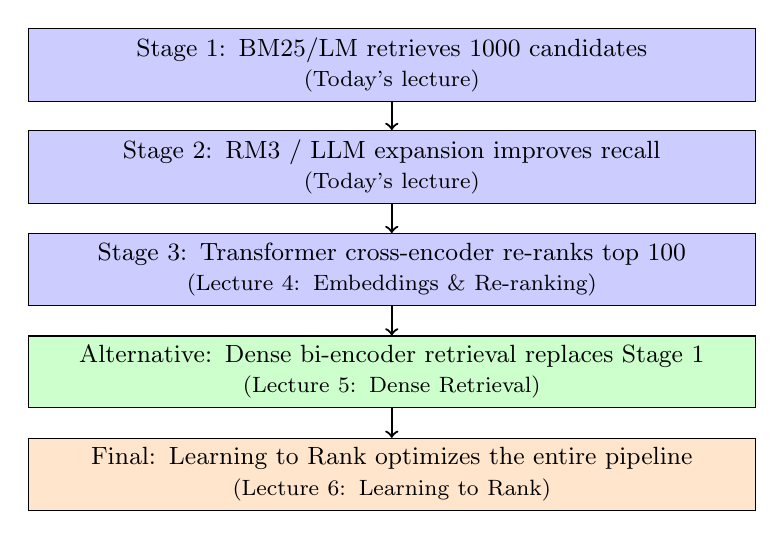
\begin{tikzpicture}[
    node distance=1.3cm,
    box/.style={rectangle, draw, fill=blue!20, text width=9cm, align=center, minimum height=0.9cm, font=\small},
    arrow/.style={->, thick}
]
    \node[box] (stage1) {Stage 1: BM25/LM retrieves 1000 candidates \\ \footnotesize (Today's lecture)};
    \node[box, below of=stage1] (stage2) {Stage 2: RM3 / LLM expansion improves recall \\ \footnotesize (Today's lecture)};
    \node[box, below of=stage2] (stage3) {Stage 3: Transformer cross-encoder re-ranks top 100 \\ \footnotesize (Lecture 4: Embeddings \& Re-ranking)};
    \node[box, below of=stage3, fill=green!20] (alt) {Alternative: Dense bi-encoder retrieval replaces Stage 1 \\ \footnotesize (Lecture 5: Dense Retrieval)};
    \node[box, below of=alt, fill=orange!20] (final) {Final: Learning to Rank optimizes the entire pipeline \\ \footnotesize (Lecture 6: Learning to Rank)};
    
    \draw[arrow] (stage1) -- (stage2);
    \draw[arrow] (stage2) -- (stage3);
    \draw[arrow] (stage3) -- (alt);
    \draw[arrow] (alt) -- (final);
\end{tikzpicture}

\end{center}
\end{frame}

\begin{frame}{Preview: Lecture 4 --- Embeddings \& Transformer Re-rankers}
\begin{block}{Why Transformers?}
Sparse methods don't understand semantics:
\begin{itemize}
    \item Synonyms not recognized
    \item Polysemy not resolved
    \item Context not considered
\end{itemize}
\end{block}

\begin{block}{What You'll Learn}
\begin{itemize}
    \item Word embeddings (Word2Vec, GloVe): words as dense vectors
    \item Self-attention and the Transformer architecture
    \item BERT: contextualized embeddings for relevance
    \item Cross-encoder re-ranking: joint query-document scoring
\end{itemize}
\end{block}

\begin{exampleblock}{Connection}
Your BM25 pipeline becomes the first-stage retriever. BERT re-ranks on top.
\end{exampleblock}
\end{frame}

\begin{frame}{Why Sparse Methods Still Matter}
\begin{enumerate}
    \item \textbf{Efficiency:} BM25 in microseconds vs.\ dense in milliseconds
    
    \item \textbf{Transparency:} Explainable scores (IDF, TF contributions), debuggable
    
    \item \textbf{Hybrid Systems:} Best results combine sparse + dense (complementary)
    
    \item \textbf{First-Stage Retrieval:} Neural methods too slow for full corpus --- BM25 narrows candidates
    
    \item \textbf{Feature Engineering:} BM25, LM scores become features in Learning to Rank (Lecture 6)
\end{enumerate}

\vspace{1em}

\begin{alertblock}{Bottom Line}
BM25 is not going away. It is the \textbf{foundation layer} of every modern retrieval system.
\end{alertblock}
\end{frame}

% ====================================================================
% WRAP-UP
% ====================================================================
\section{Summary and Assignment}

\begin{frame}[plain]
\sectionpage
\end{frame}

\begin{frame}{Key Takeaways}
\begin{block}{1. BM25 is the Industry Standard}
Probabilistic foundation, robust performance. Defaults ($k_1=1.2$, $b=0.75$) work for most collections. BM25F extends to fielded documents.
\end{block}

\begin{block}{2. Query Expansion Improves Recall}
RM3 addresses vocabulary mismatch. LLM-based expansion offers zero-shot alternatives (HyDE, Query2Doc, decomposition). Watch for query drift.
\end{block}

\begin{block}{3. Language Models Provide Principled Alternative}
Generative probabilistic framework. Smoothing is essential. Dirichlet best for variable-length collections.
\end{block}

\begin{block}{4. Everything Connects}
BM25 $\to$ first-stage retriever. LM $\to$ foundation for neural LMs. RM3 $\to$ connects LM theory to expansion practice. All become features in LTR.
\end{block}
\end{frame}

\begin{frame}{Assignment: Sparse Ranking Comparison}
\textbf{Due:} Before Lecture 5

\vspace{0.5em}

\begin{block}{Part 1: Baseline Comparison (30 pts)}
Implement BM25 and Dirichlet LM. Tune parameters: 3+ values each for $k_1$, $b$, $\mu$. Report MAP, NDCG@10, P@10.
\end{block}

\begin{block}{Part 2: Query Expansion (30 pts)}
Add RM3 to your best baseline. Experiment with fb\_docs and fb\_terms. \textbf{Bonus:} Implement LLM-based expansion and compare.
\end{block}

\begin{block}{Part 3: Analysis (20 pts)}
For 3 queries, explain ranking differences between BM25 and LM. Show successful expansion and query drift examples. Discuss production trade-offs.
\end{block}

\begin{block}{Part 4: Looking Ahead (20 pts)}
Which queries would benefit from semantic matching (dense retrieval)? What features would you extract for learning to rank?
\end{block}
\end{frame}

\begin{frame}{Next Class: Embeddings \& Transformer Re-rankers}
\begin{block}{Preparation}
\textbf{Read:}
\begin{itemize}
    \item Vaswani et al.\ (2017): ``Attention Is All You Need''
    \item Nogueira \& Cho (2019): ``Passage Re-ranking with BERT''
\end{itemize}

\textbf{Skim:}
\begin{itemize}
    \item Devlin et al.\ (2019): ``BERT: Pre-training of Deep Bidirectional Transformers''
\end{itemize}
\end{block}

\vspace{0.5em}

\begin{exampleblock}{What We'll Build}
\begin{itemize}
    \item Use your BM25 pipeline as first-stage retriever
    \item Add BERT re-ranker on top
    \item Compare sparse vs.\ neural ranking
\end{itemize}
\end{exampleblock}
\end{frame}

\begin{frame}{Questions?}
\begin{center}
\Huge Questions?

\vspace{2em}

\Large
Office Hours: [Your time]

\vspace{1em}

Email: [Your email]

\vspace{2em}

\normalsize
\textbf{Good luck with the assignment!}
\end{center}
\end{frame}

% ====================================================================
% APPENDIX / BACKUP SLIDES
% ====================================================================
\appendix

\begin{frame}{Backup: BM25 Variants}
\begin{block}{BM25+}
Adds a lower bound $\delta$ on term contribution:
$$\text{BM25+}(q,d) = \sum_{t \in q} \text{IDF}(t) \cdot \left(\frac{f(t,d) \cdot (k_1+1)}{f(t,d) + k_1 \cdot \text{norm}} + \delta\right)$$
\end{block}

\begin{block}{BM25F (Details)}
Per-field weights and normalization. Common field weights:
\begin{itemize}
    \item Title: $w = 5{-}10$, Body: $w = 1$, URL: $w = 2{-}3$, Anchor: $w = 3{-}5$
\end{itemize}
\end{block}
\end{frame}

\begin{frame}{Backup: Other Smoothing Methods}
\begin{block}{Absolute Discounting}
$$P(w|d) = \frac{\max(\text{count}(w,d) - \delta, 0)}{|d|} + \frac{\delta \cdot |V_d|}{|d|} \cdot P(w|C)$$
Subtracts fixed discount $\delta$ from each count; redistributes to unseen words.
\end{block}

\begin{block}{Two-Stage Smoothing}
Combine Dirichlet (document-level) + JM (collection-level). Can improve but more complex.
\end{block}
\end{frame}

\begin{frame}{Backup: HyDE Full Pipeline}
\begin{center}
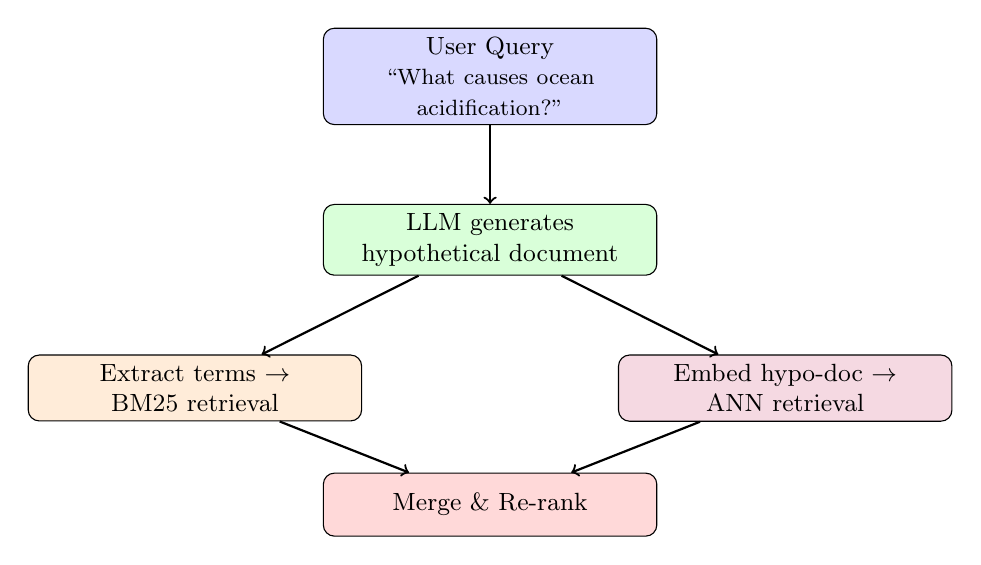
\begin{tikzpicture}[
    node distance=1cm,
    box/.style={rectangle, draw, rounded corners, text width=4cm, align=center, minimum height=0.8cm, font=\small},
    arrow/.style={->, thick}
]
    \node[box, fill=blue!15] (query) {User Query\\\footnotesize ``What causes ocean acidification?''};
    \node[box, fill=green!15, below=of query] (llm) {LLM generates\\hypothetical document};
    \node[box, fill=orange!15, below left=1cm and -0.5cm of llm] (sparse) {Extract terms $\to$\\BM25 retrieval};
    \node[box, fill=purple!15, below right=1cm and -0.5cm of llm] (dense) {Embed hypo-doc $\to$\\ANN retrieval};
    \node[box, fill=red!15, below=2.5cm of llm] (merge) {Merge \& Re-rank};
    
    \draw[arrow] (query) -- (llm);
    \draw[arrow] (llm) -- (sparse);
    \draw[arrow] (llm) -- (dense);
    \draw[arrow] (sparse) -- (merge);
    \draw[arrow] (dense) -- (merge);
\end{tikzpicture}

\end{center}
\end{frame}

\begin{frame}{Backup: Rocchio vs. RM3 vs. LLM Expansion}
\begin{table}
\centering
\footnotesize
\begin{tabular}{lccc}
\toprule
\textbf{Aspect} & \textbf{Rocchio} & \textbf{RM3} & \textbf{LLM-Based} \\
\midrule
Foundation & Geometric & Probabilistic & Neural generative \\
Term selection & All (weighted) & Top-$k$ by $P(w|R)$ & Prompted generation \\
Knowledge source & Retrieved docs & Retrieved docs & Parametric \\
Failure mode & Noisy centroid & Query drift & Hallucination \\
Cold start & Needs corpus & Needs corpus & Works zero-shot \\
Cost & Free & Free & API / GPU \\
Performance & Good & Better & Context-dependent \\
Era & 1971 & 2001 & 2023+ \\
\bottomrule
\end{tabular}
\end{table}
\end{frame}

\end{document}